% !TeX document-id = {2870843d-1baa-4f6a-bd0a-a5c796104a32}
% !BIB TS-program = biber
% !TeX encoding = UTF-8
% TU Delft beamer template

\documentclass[aspectratio=169,small]{beamer}
\usepackage[english]{babel}
\usepackage{csquotes}
\usepackage{calc}
\usepackage[absolute,overlay]{textpos}
\usepackage{graphicx}
\usepackage{subfig}
\usepackage{mathtools}
\usepackage{amsfonts}
\usepackage{amsthm}
\usepackage{comment}
\usepackage{siunitx}
\usepackage{MnSymbol,wasysym}
\usepackage{array}
\usepackage{qrcode}
\usepackage{tikz}

\setbeamertemplate{navigation symbols}{} % remove navigation symbols
\mode<presentation>{\usetheme[verticalbar=false]{tud}}

% BIB SETTINGS
\usepackage[
    backend=biber,
    giveninits=true,
    maxnames=30,
    maxcitenames=20,
    uniquename=init,
    url=false,
    style=authoryear,
]{biblatex}
\addbibresource{bibfile.bib}
\setlength\bibitemsep{0.3cm} % space between entries in the reference list
\renewcommand{\bibfont}{\normalfont\scriptsize}
\setbeamerfont{footnote}{size=\tiny}
\renewcommand{\cite}[1]{\footnote<.->[frame]{\fullcite{#1}}}
\setlength{\TPHorizModule}{\paperwidth}
\setlength{\TPVertModule}{\paperheight}

\newcommand{\absimage}[4][0.5,0.5]{%
	\begin{textblock}{#3}%width
		[#1]% alignment anchor within image (centered by default)
		(#2)% position on the page (origin is top left)
		\includegraphics[width=#3\paperwidth]{#4}%
\end{textblock}}

\newcommand{\mininomen}[2][1]{{\let\thefootnote\relax%
	\footnotetext{\begin{tabular}{*{#1}{@{\!}>{\centering\arraybackslash}p{1em}@{\;}p{\textwidth/#1-2em}}}%
	#2\end{tabular}}}}


% to solve spurious empty pages before a frame containing footnotes
\setbeamertemplate{footnote}{%
  \makebox[1em][l]{\insertfootnotemark}%
  \begin{minipage}{\dimexpr\linewidth-1em}
    \usebeamerfont{footnote}\insertfootnotetext
  \end{minipage}\vskip 0pt}


\title[]{External flow Boundary Conditions}
\institute[]{Delft University of Technology, The Netherlands}
\author{G D Weymouth \and M Lauber}
\date{}

\begin{document}
\section{Introduction}
{
\setbeamertemplate{footline}{\usebeamertemplate*{minimal footline}}
\frame{\titlepage}
}

\begin{frame}[fragile]{WaterLily is memory limited} % some commands, e.g. \verb require [fragile]
  \begin{columns}[onlytextwidth]
  \begin{column}{.5\textwidth}
    \vspace{1cm}
    \begin{itemize}
      \item TGV with $N=128^3$ in 15min on laptop
      \item Need a supercomputer to do $N=256^3$
    \end{itemize}
    \vspace{1cm}
  \vfill
  \begin{block}{Options}<2->
    \begin{itemize}
      \item MPI + CUDA 
      \item<3-> Use smaller domains with better BCs
    \end{itemize}
  \end{block}
  \end{column}
  \begin{column}{.5\textwidth}
    \absimage{.73, .45}{.40}{fig/draw2.png}
  \end{column}
  \end{columns}
\end{frame}


\begin{frame}[fragile]{Reflection BCs waste cells} % some commands, e.g. \verb require [fragile]
  \begin{columns}[onlytextwidth]
  \begin{column}{.5\textwidth}
    \vspace{1cm}
    \begin{itemize}
      \item Avoiding blockage requires $Ny\approx Nz\approx 10L$ and $Nx\approx 5L$ in front
      \item Grid stretching has limits and still requires cells!
    \end{itemize}
    \vspace{1cm}
  \begin{alertblock}{Need non-blocking BC}
      Using $N=(2L)^3$ would be 125x speed up!
  \end{alertblock}
  \end{column}
  \begin{column}{.5\textwidth}
    \absimage{.73, .45}{.40}{fig/draw2.png}
  \end{column}
  \end{columns}
\end{frame}

\begin{frame}[fragile]{Reflection BCs are cheaper than needed} % some commands, e.g. \verb require [fragile]
  \begin{block}{Integrate}
      \begin{align*}
        &u^* = \mu_0(u^0+R_{\Delta t})+(1-\mu_0)U_b &\quad\forall\ x\in\Omega (N) \\
        &\partial u^*_s/\partial n = 0,\ u^*_n = U_n &\quad\forall\ x\in\partial\Omega (N^{1/2})
      \end{align*}
  \end{block}
  \begin{block}{Project}
      \begin{align*}
          &\nabla\cdot\mu_0\nabla p = \nabla\cdot u^* &\quad\forall\ x\in\Omega (N)\\
          &u = u^*-\mu_0\nabla p &\quad\forall\ x\in\Omega (N)\\
          &\partial u_s/\partial n = 0,\ u_n = U_n &\quad\forall\ x\in\partial\Omega (N^{1/2})
      \end{align*}
  \end{block}
  Is there a $\partial\Omega$ equation to reduce blockage with $O(N)$ cost?
\end{frame}

\begin{frame}[fragile]{Biot-Savart for irrotational external flow} % some commands, e.g. \verb require [fragile]
    \begin{align*}
      u(x) = f(x,\omega) = \int_{\only<1>{\color{red}\infty}\only<2->\Omega} \frac{\omega(x')\times(x-x')}{2\pi|x-x'|^2}dx'\\
    \end{align*}
    \vspace{-1cm}
    \begin{itemize}
      \item<2-> Assume all vorticity is within $\Omega$ and compute $\omega$ once $O(N)$
      \item<3-> Compute $u$ integral $O(N)$ for each boundary point $O(N^{1/2})$
      \only<5>{\vspace{-2mm}\hline\vspace{2mm}}
      \item<5> Compute $u$ integral {\color{teal}$O(\ln N)$} for each boundary point $O(N^{1/2})$
    \end{itemize}
  \begin{alertblock}{$O(N^{3/2})$ is too slow}<4->
     Need faster integral method!
  \end{alertblock}
  \begin{exampleblock}{$O(N^{1/2}\ln N )$ would be great!}<5>
     How can we compute the integral that fast?
  \end{exampleblock}
\end{frame}

\begin{frame}[fragile]{Multi-level pooling achieves $O(\ln N)$ integration} % some commands, e.g. \verb 
    \absimage{.25, .42}{.5}{fig/full_vort.png}
    \absimage{.75, .42}{.5}{fig/multilevel_vort.png}
    \vspace{52mm}
    \begin{itemize}
        \item $\omega$ is progressively pooled through $O(\ln N)$ levels ahead of time
        \item $f(x)$ uses $\omega(x')$ from low levels for large $|x-x'|$, minimizing error
        \item Zero allocations and $O(1)$ operations on each level 
    \end{itemize}
\end{frame}

\begin{frame}[fragile]{Momentum using Biot-Savart BCs} % some commands, e.g. \verb require [fragile]
  \begin{block}{Integrate}
      \begin{align*}
        &u^* = \mu_0(u^0+R_{\Delta t})+(1-\mu_0)U_b &\quad\forall\ x\in\Omega\ O(N) \\
        &u^* = f(x_\partial,\nabla\times u^*) &\quad\forall\ x_\partial\in\partial\Omega\ O(N)
      \end{align*}
  \end{block}
  \begin{block}{Project}
      \begin{align*}
          &\nabla\cdot\mu_0\nabla p = \nabla\cdot u^*\only<3>{\color{teal}{-\nabla\cdot f(x_\partial,\nabla\times\mu_0\nabla p)}} &\quad\forall\ x\in\Omega\only<3>{, x_\partial\in\partial\Omega}\ O(N)\\
          &u = u^*-\mu_0\nabla p &\quad\forall\ x\in\Omega\ O(N)\\
          &u \only<1>{ = f(x,\nabla\times u)}= u^*-f(x_\partial,\nabla\times\mu_0\nabla p) &\quad\forall\ x_\partial\in\partial\Omega\ O(N)
      \end{align*}
  \end{block}
  \begin{alertblock}{Pressure couples body and $\partial\Omega$}<2>
    Pressure does not induce divergence free velocity!
  \end{alertblock}
  \vspace{-15mm}
  \begin{exampleblock}{Pressure couples body and $\partial\Omega$}<3>
    Updating Poisson solver source each iteration ensures $\nabla\cdot u = 0$
  \end{exampleblock}
\end{frame}

\begin{frame}[fragile]{Results confirm that reflection requires a big domain....} % some commands, e.g. \verb 
    \small{Impulsively started circle with $D=3L/4$: inline velocity $u$}
    
    \begin{columns}[onlytextwidth]
        \begin{column}{.5\textwidth}
        \begin{figure}
            \centering
            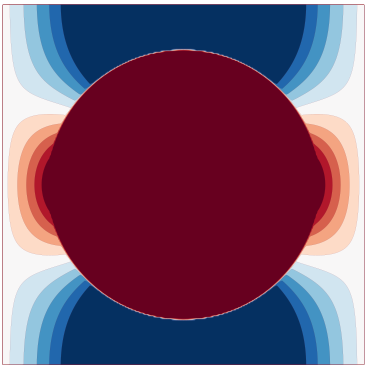
\includegraphics[height=0.6\textwidth]{fig/reflection_tight.png}
            \caption*{Reflection BCs: \\ \color{red}{$u_\text{max}=4.36U$, 13 Poisson it}}
        \end{figure}
        \end{column}
        \begin{column}{.5\textwidth}<2->
        \begin{figure}
            \centering
            \includegraphics<2>[height=0.6\textwidth]{fig/reflection_big.png}
            \includegraphics<3>[height=0.6\textwidth]{fig/reflection_zoom.png}
            \caption*{Reflection {\color{red}$8\times$size}: \\ $u_\text{max}=1.97U$, {\color{red} 15 it, 70x time}}
        \end{figure}
        \end{column}
    \end{columns}
\end{frame}

\begin{frame}[fragile]{Biot-Savart BCs are \textit{faster} than reflection} % some commands, e.g. \verb 
    \small{Impulsively started circle with $D=3L/4$: inline velocity $u$}    
    \begin{columns}[onlytextwidth]
        \begin{column}{.5\textwidth}
        \begin{figure}
            \centering
            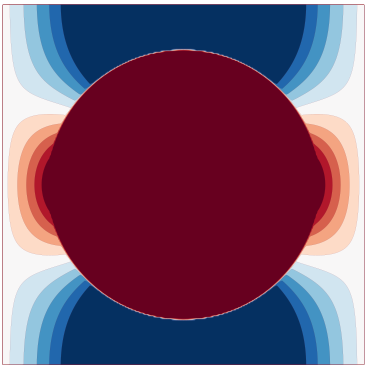
\includegraphics[height=0.6\textwidth]{fig/reflection_tight.png}
            \caption*{Reflection BCs: \\ \color{red}{$u_\text{max}=4.36U$, 13 Poisson it}}
        \end{figure}
        \end{column}
        \begin{column}{.5\textwidth}
        \begin{figure}
            \centering
            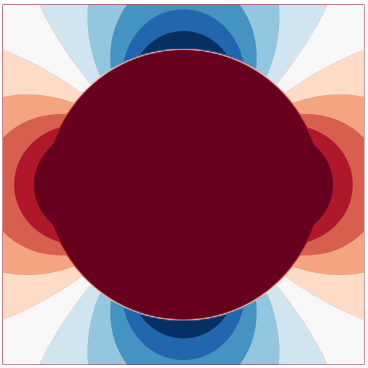
\includegraphics[height=0.6\textwidth]{fig/biotBC.png}
            \caption*{Biot-Savart BCs: \\ \color{teal} {$u_\text{max}=2.01U$, 8 it, 0.95time}}
        \end{figure}
        \end{column}
    \end{columns}
\end{frame}

\begin{frame}[fragile]{Biot-Savart BCs are \textit{MUCH faster} than reflection} % some commands, e.g. \verb 
    \small{$Re=10^4$ circle @ $t=2D/U$: vorticity $\omega$} 
    \begin{columns}[onlytextwidth]
        \begin{column}{.5\textwidth}
        \begin{figure}
            \centering
            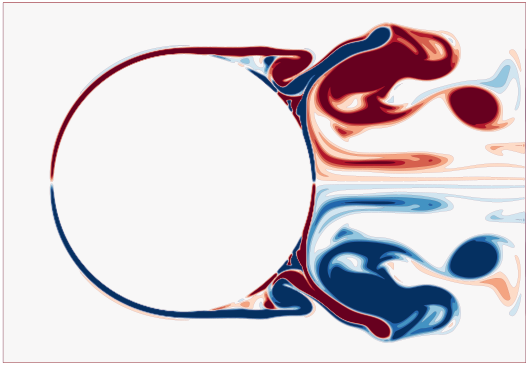
\includegraphics[height=0.6\textwidth]{fig/reflect_Re1e4_sim.png}
            \caption*{Reflection BCs: \\ Large $u$ leads to small $\Delta t$}
        \end{figure}
        \end{column}
        \begin{column}{.5\textwidth}
        \begin{figure}
            \centering
            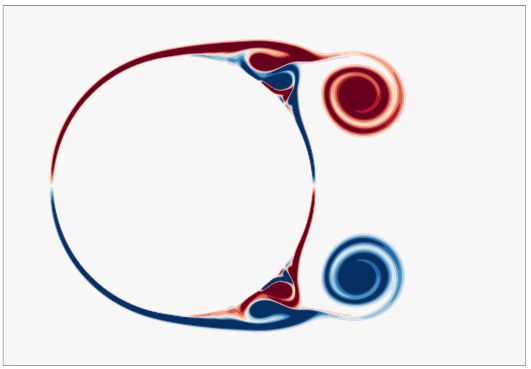
\includegraphics[height=0.6\textwidth]{fig/biot_Re1e4_sim.png}
            \caption*{Biot-Savart BCs: \\ 2x speed-up!}
        \end{figure}
        \end{column}
    \end{columns}
\end{frame}

\begin{frame}[fragile]{Biot-Savart BCs remove domain dependence} % some commands, e.g. \verb 
    \begin{columns}[onlytextwidth]
        \begin{column}{.5\textwidth}
        \begin{figure}
            \centering
            \includegraphics<1>[height=0.7\textwidth]{fig/start.png}
            \includegraphics<2>[height=0.7\textwidth]{fig/fft.png}
        \end{figure}
        \end{column}
        \begin{column}{.5\textwidth}
        \begin{figure}
            \centering
            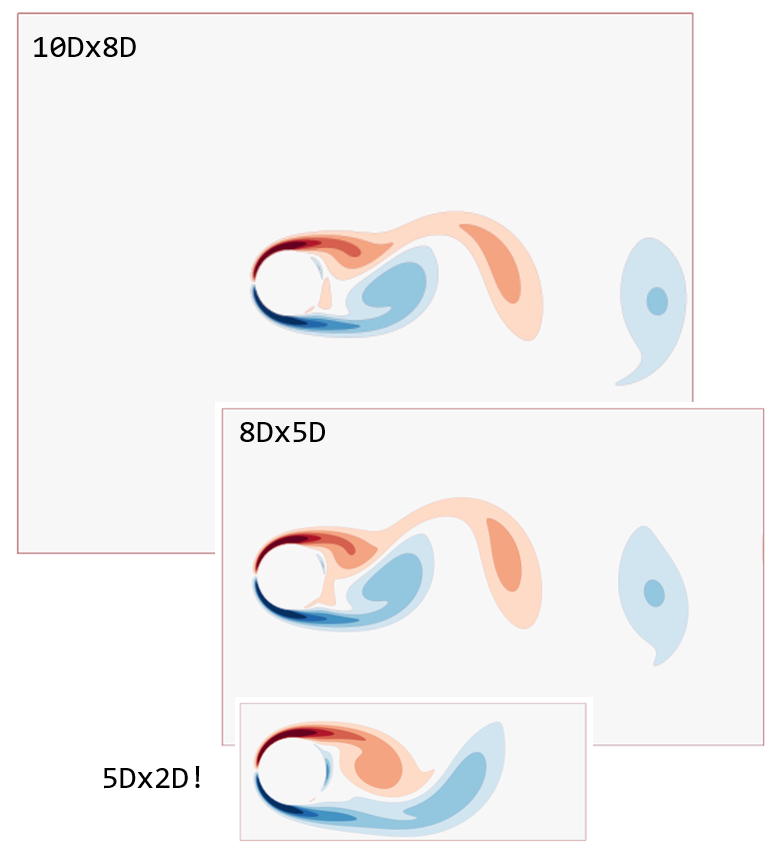
\includegraphics[height=0.95\textwidth]{fig/domains.png}
        \end{figure}
        \end{column}
    \end{columns}
\end{frame}


\begin{frame}[fragile]{Biot-Savart BCs replicate non-trivial results} % some commands, e.g. \verb 
    \begin{figure}
        \centering
        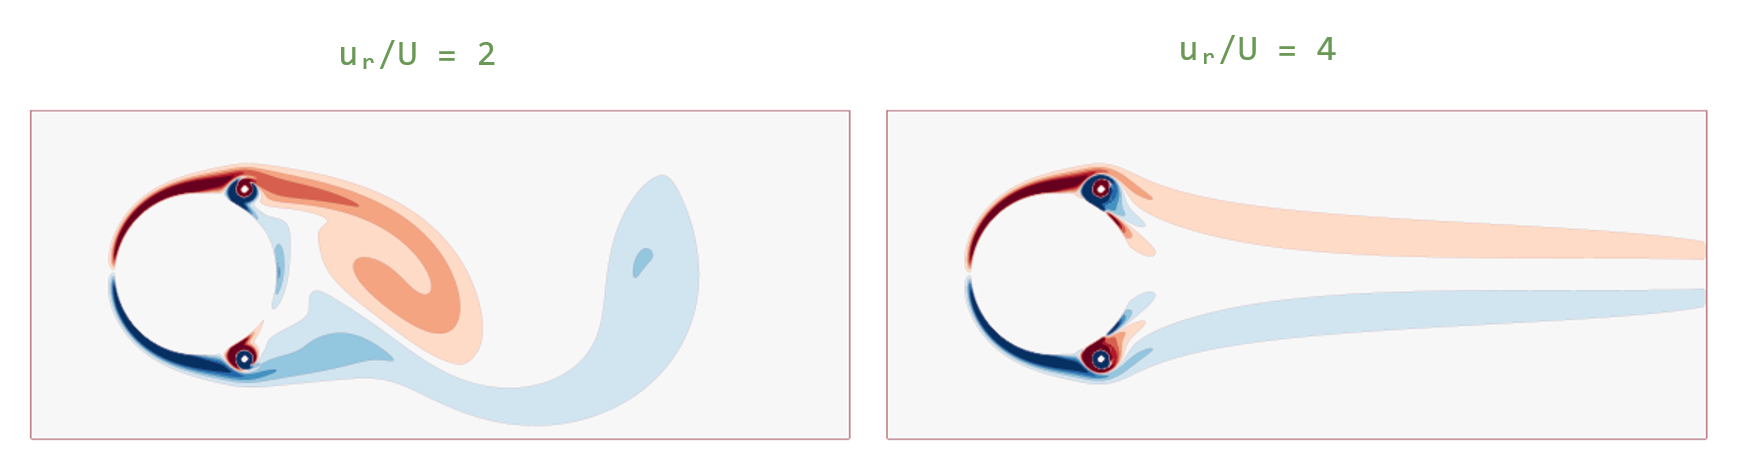
\includegraphics[width=\textwidth]{fig/spinning cylinders.png}
    \end{figure}
    \begin{itemize}
        \item Two small spinning cylinders to control large cylinder wake
        \item $Re_D=500,\ d/D=10\%,\ \theta=120\deg,\ \text{gap}/D=5\%$
        \item Steady wake for $u_r/U>3$ matches Schulmeister et al \textit{JFM}, 2017
    \end{itemize}
\end{frame}

% \begin{frame}{Mass--energy equivalence}
% 	They say every formula you add to a presentation, will reduce your audience by \SI{50}{\percent}. A simple yet effective way to mitigate this effect, is adding a compact nomenclature to the slides containing formulae.
	
% 	\[E=mc^2\]
	
% 	If you find this is taking up too much of your precious space, than you are doing something wrong, and it is not adding this little nomenclature.
	
% 	The optional argument specifies the number of column pairs.
	
% \mininomen[2]{% number of columns
%   $E$ & Energy (\unit{J})                     & $m$ & Mass (\unit{kg}) \\
%   $c$ & Speed of light in vacuum (\unit{m/s})
%   }
% \end{frame}

% \begin{frame}
%   Thanks for your attention.

%   A digital version of this presentation can be found here:
%   \vfill
%   \url{https://gitlab.com/novanext/tudelft-beamer} 
%   \vfill  
%   \centering
%   \qrcode{https://gitlab.com/novanext/tudelft-beamer}
%   \vfill
% \end{frame}

% \begin{frame}[allowframebreaks,t]{\bibname}
% 	% the 'I' is caused by 'allowframebreaks'
% 	\AtNextBibliography{\footnotesize}% or in the preamble \AtBeginBibliography{\small}
% 	\printbibliography
% \end{frame}


\end{document}

